\documentclass[17pt]{article}

\usepackage[margin=1in, paperwidth=8.5in, paperheight=11in]{geometry}
\usepackage{amsmath}
\usepackage[document]{ragged2e}
\usepackage{graphicx}
\usepackage{listings}
\usepackage{color}
\usepackage[none]{hyphenat}


\definecolor{dkgreen}{rgb}{0,0.6,0}
\definecolor{gray}{rgb}{0.5,0.5,0.5}
\definecolor{mauve}{rgb}{0.58,0,0.82}

\lstset{frame=tb,
  language=Matlab,
  aboveskip=3mm,
  belowskip=3mm,
  showstringspaces=false,
  columns=flexible,
  basicstyle={\small\ttfamily},
  numbers=none,
  numberstyle=\tiny\color{gray},
  keywordstyle=\color{blue},
  commentstyle=\color{dkgreen},
  stringstyle=\color{mauve},
  breaklines=true,
  breakatwhitespace=true,
  tabsize=3
}



\begin{document}

\title{{Exercise 1}}
\author{Dejan Porjazovski}
\maketitle


\section{Question 1}
\begin{itemize}
	\item{What are the properties of MFCC features that make them well 			suited for automatic speech recognition?}
\end{itemize}
The MFCC decorrelates the features and reduces the dimensionality, which
makes them suited for automatic speech recognition. \\
It uses linear filter banks on lower frequencies and increases bin size on higher frequencies.

\begin{itemize}
	\item{Why spectrogram or mel-spectrum wouldn't work so well?}
\end{itemize}
The power spectrogram contains a lot of data and redundancy. It also
contains a lot of noise. \\
The mel spectrogram is better. It contains approximately 10 times less data. It also contains less noise and less redundancy compared to the power spectrogram. \\
MFCC uses discrete cosine transformation in order to decorrelate the
features and reduce the dimensionality and is the most used method.


\begin{align}
\textbf{SOURCE CODE}
\end{align}

\begin{lstlisting}
addpath /work/courses/T/S/89/5150/general/ex1
addpath /work/courses/T/S/89/5150/general/ex1/gmmbayestb
load ex1data

plot(sampleword);


s = spectrogram(sampleword, hamming(400), 240);
imagesc(sqrt(abs(s)))
axis xy
sample_word_segmentation


s2 = spectrogram(filter([1 -0.97], 1, sampleword), hamming(400), 240);
figure
imagesc(sqrt(abs(s2)))
axis xy
sample_word_segmentation


plot(M', 'b')


figure
imagesc(log(M*sqrt(abs(s2))+1))
axis xy
sample_word_segmentation


imagesc(D)
colorbar


figure
imagesc(D*log(M*sqrt(abs(s2))+1))
axis xy
sample_word_segmentation
\end{lstlisting}


\section{Question 2}
\begin{itemize}
	\item{Plot the error rates of both the train and the test sets with respect to the number of components in GMMs.}	
\end{itemize}


\begin{center}
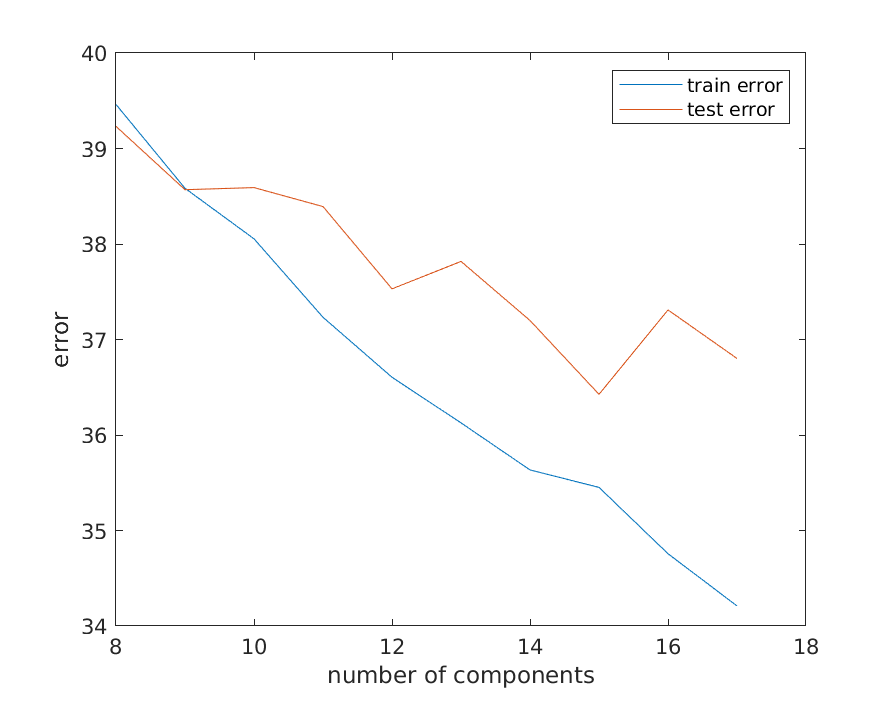
\includegraphics[width=15cm, height=8cm]{error.png}
\end{center}

\begin{itemize}
	\item{Why are the recognition results with the train and the test set different?}
\end{itemize}
The results are different because the classifier is trained on the training data and that is why is has lower error rate. \\
On the other hand, the test set data has not been seen previously by the
classifier, so that is why it performs worse on it.

\begin{itemize}
	\item{What is a good number of components for recognizing an unknown set of samples?}
\end{itemize}
From the plot we can see that the optimal number of components for
recognizing an unknown set of samples is 15.

\newpage
\begin{align}
\textbf{SOURCE CODE}
\end{align}

\begin{lstlisting}
addpath /work/courses/T/S/89/5150/general/ex1
addpath /work/courses/T/S/89/5150/general/ex1/gmmbayestb
load ex1data

error = [];
error_test = [];
num_components = [];

for i = drange(8:17)
    S = train_gmm(train_data, train_class, i);
    result = gmmb_decide(gmmb_normalize(gmmb_pdf(train_data, S)));
    %phonemes(result(2991:3010))
    error = [error, length(find(result~=train_class))/length(train_class)*100];

    result_test = gmmb_decide(gmmb_normalize(gmmb_pdf(test_data, S)));
    error_test = [error_test, length(find(result_test~=test_class))/length(test_class)*100];
    
    num_components = [num_components, i];
end

figure1 = figure;
plot(num_components, error)
hold on;
plot(num_components, error_test)
hold off;
legend({'train error', 'test error'});
xlabel('number of components');
ylabel('error');
\end{lstlisting}


\section{Question 3}
\begin{itemize}
	\item{Based on the confusion matrix, what can you conclude about phoneme recognition as a task and recognition performance of different phoneme classifiers?
}
\end{itemize}
Based on the confusion matrix, we can say that the classifier did fairly
well recognizing the phonemes. \\
The model did best recognizing the phonemes 's' and 'u'.

\begin{itemize}
	\item{Give examples of difficulties this classifier has.}
\end{itemize}
The classifier had difficulties recognizing 'p', 't', 'k'. \\
It mostly struggles recognizing the unvoiced phones.

\begin{itemize}
	\item{Include the visualized confusion matrix with the answer.}
\end{itemize}
\begin{center}
	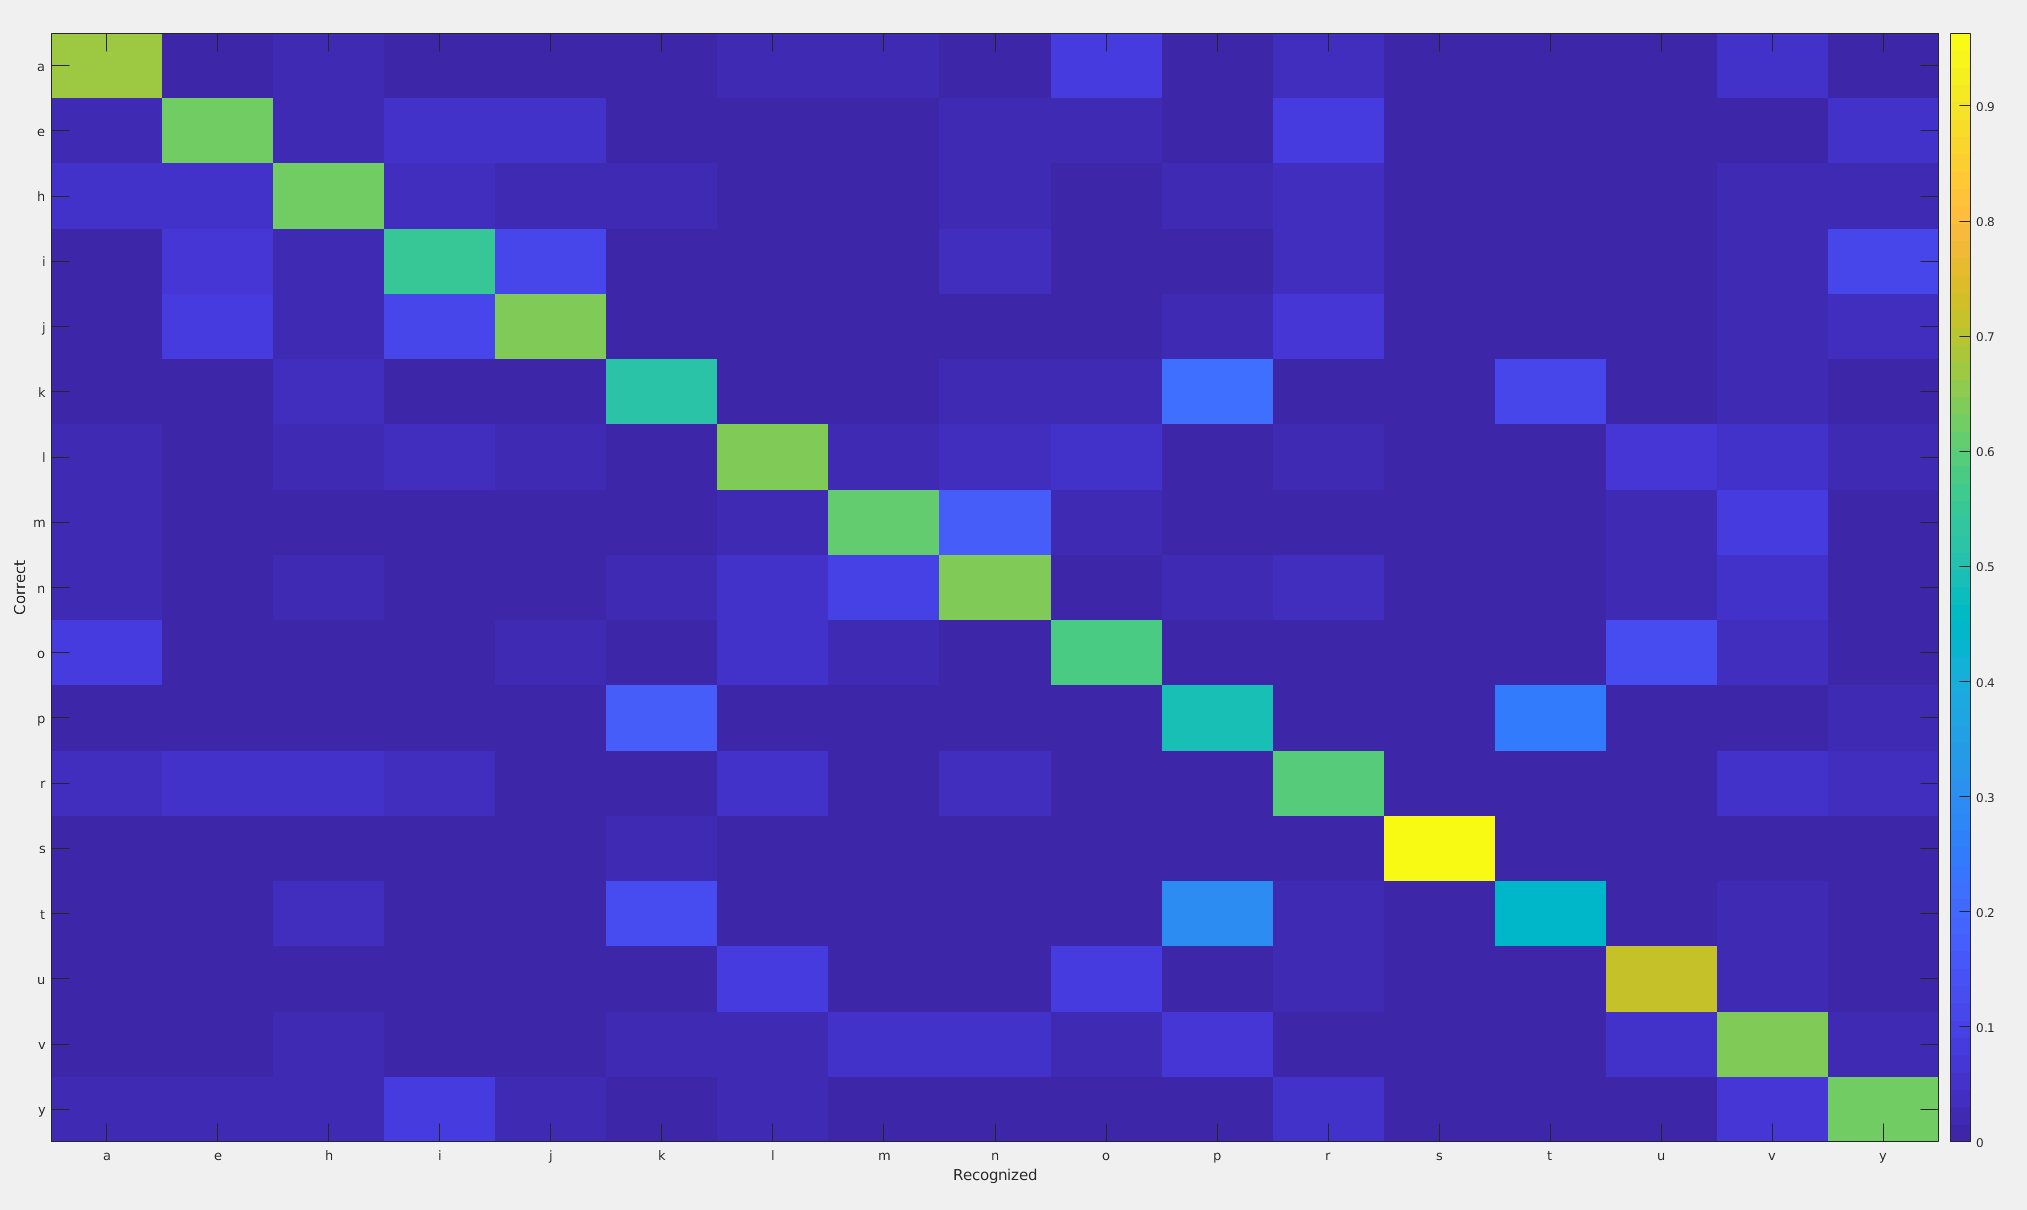
\includegraphics[width=18cm, height=10cm]{confusion_matrix.png}
\end{center}


\begin{align}
\textbf{SOURCE CODE}
\end{align}

\begin{lstlisting}
addpath /work/courses/T/S/89/5150/general/ex1
addpath /work/courses/T/S/89/5150/general/ex1/gmmbayestb
load ex1data


S = train_gmm(train_data, train_class, 15);

result_test = gmmb_decide(gmmb_normalize(gmmb_pdf(test_data, S)));
error_test = length(find(result_test~=test_class))/length(test_class)*100;

C = confusion_matrix(result_test, test_class);

plot_confusion(C, phonemes);
\end{lstlisting}


\section{Question 4}
\begin{itemize}
	\item{What problems do you see in the frame based classification if one wants to recognize whole words?}
\end{itemize}
It doesn't work well for recognizing whole words because it repeats the same phoneme many times and also if it misclassifies a phoneme, the word might change it's meaning.
For example for the first word (tw1) I got: \\~\\
'ttptkkpkttpptkkkkkkkooooooooollllllloolmmmmmmmmiiieeeeeyt' \\~\\
I don't know Finnish that much but this might be the word 'kolme'. \\~\\
The second word looks like this: \\~\\
'sssssssssssssssseeeeeeeeeeeeyiiyyiiiiiyiiiisssssssssssssssssstt'
\\~\\
The third word looks like this: \\~\\
'hrhhhyereeeeeeellllirnnmmmmmvvviiiykktttkkkukouuuuuuuuuuuussssssssssssssstavaaaaoaavaon
'

\begin{itemize}
	\item{Describe ideas to improve the results.}
\end{itemize}
One idea would be to increase the number of GMM components because I am using 15, which gave me the lowest error but that might be local minimum. \\
We can also gather more data and maybe use different speakers.
\\
Another idea for word recognition would be to use some kind of windowing to separate te word and find the most common phoneme in each window.



\begin{align}
\textbf{SOURCE CODE}
\end{align}

\begin{lstlisting}
addpath /work/courses/T/S/89/5150/general/ex1
addpath /work/courses/T/S/89/5150/general/ex1/gmmbayestb
load ex1data

S = train_gmm(train_data, train_class, 15);


tw1_predict = gmmb_decide(gmmb_normalize(gmmb_pdf(tw1, S)));
first_word = [];

for i = drange(1, length(tw1_predict))
   first_word = [first_word, phonemes(tw1_predict(i))];
end
first_word


tw2_predict = gmmb_decide(gmmb_normalize(gmmb_pdf(tw2, S)));
second_word = [];

for i = drange(1, length(tw2_predict))
   second_word = [second_word, phonemes(tw2_predict(i))];
end
second_word



tw3_predict = gmmb_decide(gmmb_normalize(gmmb_pdf(tw3, S)));
third_word = [];

for i = drange(1, length(tw3_predict))
   third_word = [third_word, phonemes(tw3_predict(i))];
end
third_word

\end{lstlisting}


\section{Bonus Question 1}
\begin{itemize}
	\item{Which model performs classification better, the DNN or your best GMM?}
\end{itemize}
The results are similar but DNN model performs slightly better than GMM.
With more data, the DNN model should outperform the GMM with a lot more difference.

\begin{itemize}
	\item{The DNN training script tells you the number of parameters. Look inside your best model (struct S in Matlab). Which has more parameters? }
\end{itemize}
The GNN model has 17 parameters and the DNN model has 145707.


\section{Bonus Question 2}
\begin{itemize}
	\item{Which model has lower classification error on the sampled MFCCs? Why might that be?}
\end{itemize}
The DNN model has lower classification error which is 31.3\% compared to 37\% in the GNN model. \\~\\
That might be because DNN model has a lot more parameters than the GNN model so it learns more about the data and thus has lower error.
  

\end{document}










